\chapter{PEM Algorithms}~\label{PEM}

In this part, we will present a review of different and classical algorithms in the PEM model of computation. We will start by presenting the general purpose algorithms, those that serve as building blocks for many other problems. We will follow by those who are related to graphs and their inherent complexity, then will come those related to more geometric problems. We will then present the algorithms linked to the matrices and finally we will come back to sorting ones due to their capital importance.

We would like to emphasize that the PEM computation model focuses on the number of blocks transferred between a supposedly large and slow external memory and a small and fast internal one since the idea is that making a memory request is longer than making a computation. The parallel aspect is translated by several processors, each having their own internal memory and being able to communicate between them through the external memory. Each cache is of size $M$, is partitioned in blocks of size $B$ and is exclusive to each processor, i.e., processors cannot access other processors' caches. To
perform any operation on the data, a processor must have the data in its own cache and the data is transferred between the main memory and the cache in blocks of size $B$.

The parameters are as follows:
\begin{itemize}[label={}]
    \item $N$ is the problem size.
    \item $M$ is the internal memory\index{Cache} size.
    \item $B$ is the block\index{Block} transfer size.
    \item $P$ is the number of processors.
\end{itemize}

\begin{figure}[!htb]
    \centering
    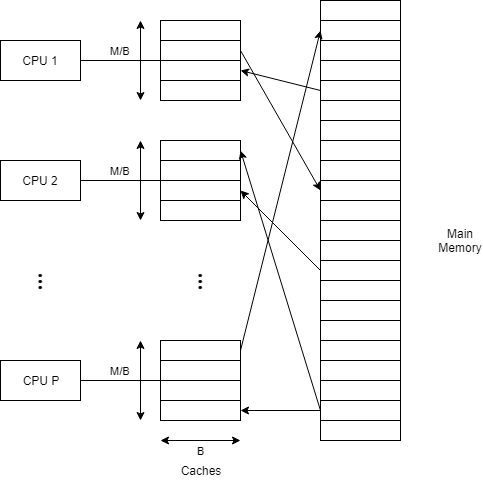
\includegraphics[width=0.4\linewidth]{Chapters/GPU/PEM.png} 
    \caption{PEM model}
\end{figure}

The model complexity measures the number of parallel block transfers between the main memory and the cache by the processors. For instance, an algorithm reading one block (or different) with each of the $P$ processors simultaneously from the main memory would have an I/O complexity of $O(1)$ and not $O(P)$.

Many of the following algorithms will have the assumption that $M \geq B^{O(1)}$ (or its weaker version $M = \Omega(B^{1 + \epsilon})$). This is called the tall-cache assumption, G.S. Brodal and R. Fagerberg prove that without the tall-cache assumption, sorting cannot be performed optimally and permuting elements is not cache-oblivious even under this property~\cite{brodal2003limits}.


\section{General purpose algorithms}

We will start by introducing different proven properties for general purpose algorithms. These typically serve as primitives for many other algorithms and their study therefore provides a solid basis for dealing with more complex problems. It is therefore all the more important to have efficient algorithms for them.

\subsection{Scanning}

Scanning is the basic operation which consists simply in consulting each of the elements in a contiguous collection in memory. Naturally, its complexity is bounded by $O(\frac{N}{PB})$. The same applies if we run several scans in parallel, like reversing the input.

\subsection{Searching}

Searching for an item in a sorted collection benefits relatively little from parallelism. Indeed, we can use an argument related to information theory, if there are $N$ elements, our element can be found in $N$ positions, so we need $\Omega(\log N)$ bits of information. And when we read a block\index{Block}, we get $\Omega(\log B)$ bits of information at once, since each block read reveals atomically where the query element fits among those B elements. In our computation model, we are able to read $P$ block\index{Block} simultaneously. Unfortunately, these are not entirely independant since they form an order and many of them will not add more information, this leads to $\Omega(\frac{\log N}{\log PB})$. 

% see: https://www.researchgate.net/profile/Jeffrey_Vitter/publication/2456841_External_Memory_Algorithms_and_Data_Structures/links/0046351d31a4390892000000/External-Memory-Algorithms-and-Data-Structures.pdf

\subsection{Permutation}

% Red blue pebble game: http://128.148.32.110/courses/csci2560/lectures/lect.16.MemoryHierarchyI.pdf
% or p.37 of greiner

Permuting data consists to rearrange all the elements into some sequence or ordre. In the PEM model, it takes asymptotically $\text{perm}_{P} (N, M, B) = \Theta(\text{min}(\frac{N}{P}, \frac{N}{PB} \log_{d} \frac{N}{B}))$ where $d$ is $\text{max}(2, \text{min}(\frac{M}{B}, \frac{N}{PB}))$~\cite{greiner2012sparse}. This result was achieved through extending the problem of bit-matrix-multiply/complement (BMMC) to PEM model of computation. Those BMMC permutations~\cite{cormen1998asymptotically} map a source index to a target index by an affine transformation over GF(2), where the source and target indices are treated as bit vectors. This class of permutations appear in several other theoretical problems as sorting, matrix transposition or Fast Fourier Transform.

But, the same argument can be done with a combinatorial extension based on the same argument that A. Aggarwal and J. S. Vitter~\cite{aggarwal1988input} or with the red blue pebble game of J. W. Hong and H. T. Kung~\cite{jia1981complexity}. Other demonstrations are also presented by G. Greiner~\cite{greiner2012sparse}, notably based on a potential function or on program traces.

The first term represents the case where we simply apply the PRAM algorithm ignoring blocks\index{Block}, each time we want to place an element, we may ask to transfer a new block\index{Block}; the second term may correspond to sorting the elements according to some indices.

\subsubsection{Hong and Kung}

They present a method to obtain lower bounds on the I/O complexity which is based on the computation graph of the algorithm. The computation graph is a directed acyclic graph (DAG) where each node $v$ corresponds to either an input (if the node $v$ does not have any ingoing edges) or either to a computation operation and its related result. An edge represents the depedency of operands.

The idea is to play a game, so called ``red-blue pebble'', on the computation graph based on some rules. A red pebble represents memory in cache\index{Cache} and blue in external. We can put a blue on top of a red or vice-versa which represents a data transfer. We need to have all red pebbles on ingoing edges to compute a new red pebble, we can remove pebbles at any time and we can have at most $M$ red pebbles on the graph. The goal of the game consists to cover some output nodes with blue pebbles according to some blue distribution at start.

They proved that a partitioning of the computation graph yields to a lower bound on the number of I/O operations. Any partition set may have a dominating set (nodes from which there exists a path from the input nodes to this set, the execution flow) of size at most $2M$. And there exists at most $\mathcal{P}(2M)$\footnote{Power set} sets and thus the minimal number of I/Os is at most $M (\mathcal{P}(2M) - 1)$. You can convince yourself that the number of transfers is directly proportional to the total size of the memory and that the number of processors is orthogonal to these notions.

\subsubsection{Aggarwal and Vitter}

The idea is to bound the maximum number of permutations that can be produced by at most $T$ I/Os, we thus search for the worst-case number of transfers required to perform $N!$ permutations. This result is independent of the number of processors used and is directly proportional since reading two times the same block\index{Block} does not help the complexity.
Let's try to estimate the minimum number of memory transfers required. We want to get all permutations of the elements, so $N!$. Only, once we have a block\index{Block}, we can make all the permutations in it without cost and we know that there are $N/B$ blocks\index{Block}, which results in the number of:
$$\frac{N!}{B!^{\frac{N}{B}}}$$

%https://pws.yazd.ac.ir/hasheminezhad/Lecture2.pdf

Now, we have to consider what happens when we consider an input or an output of the problem. Each time a new element is considered, the same process must be performed. This action must therefore be repeated N times. We also have to remember that once we get a block\index{Block}, we'll be able to generate its permutation. So, we have to count the number of way to place the block\index{Block} in the cache\index{Cache}, which corresponds to the output order of the elements $\binom{M}{B}$ or which block\index{Block} has been read. We arrive at the relation:

$$ (N \binom{M}{B})^{T} \geq \frac{N!}{B!^{\frac{N}{B}}}$$

Now, taking the logarithm on both side and applying stirling formula, this yields to:

$$ T = \Omega(\frac{N}{B} \log_{\frac{M}{B}} \frac{N}{B}) $$


\subsection{Gather and scatter}

Gather consists to group up the information coming from different memories in a tree-like fashion into a single unit, this leads to $O(\log~P)$. Of course, we can do the opposite work and spread out one to several memories for the same complexity, this inverse operation is called scatter. We can also remark three different points. First, we can serialize those procedures, second, we need to know all the participants which would imply some order among them and, third, if we allow concurrent reads, scatter can be in $O(1)$.

\subsection{All-prefix-sum}

One of the most classical algorithm in the parallel world is the all-prefix-sum (sometimes called scan). It establishes that:\\
Given an ordered set A of N elements, the prefix-sum operation returns an ordered set B of N elements, such that $ B[i] = \sum\limits_{j=0}^{i} A[j], 0 \leqslant i < N $.

It is a primitive which appears in certain algorithms, like lexically compare strings, polynomial evaluation or radix sort, since it only requires a binary associative operator~\cite{blelloch1990prefix}. And, under the assumption that the input is contiguous in memory, the problem can be solved optimally in $\Theta(\frac{N}{PB} + \log P)$ in PEM model.

The algorithm consists in four phases: we start to compute adjacent elements as $\frac{N}{P}$ parallel sums, we then ``up-sweep'', then ``down-sweep'' and we redistribute the results. The sweep phases contribute to the $O(\log P)$ term~\cite{sengupta2008efficient}.

\begin{figure}[!htb]
    \centering
    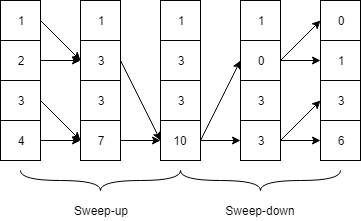
\includegraphics[width=0.5\linewidth]{Chapters/GPU/Algorithms/Belloch.png} 
    \caption{G. E. Belloch algorithm - exclusive scan}
\end{figure}


\subsection{Multiway partitioning}\label{sec:MultiwayPartitioning}

% Nice http://camlunity.ru/swap/Library/Conflux/Algorithms%20and%20Data%20Structures/gpuqsort.pdf

The multiway partitioning consists to split an unsorted set of $N$ items in $d$ bins such that all the elements in the $i$th bucket are smaller than the $d$th pivot and greater than the $d-1$th pivot given $d-1$ sorted pivots in increasing order.

This problem has most of its applications in GPU sorting~\cite{cederman2008practical}. Arge et al. proposes a more in depth analysis of the complexity in comparison to the original paper and gets: $O(\frac{N}{PB} + \lceil \frac{d}{B} \rceil \log P + d \log B)$.

The idea is a quite natural. We divide the initial vector in subelements, where we launch our processes. Each processor counts the number of elements smaller/greater than its relative pivot. Then, we compute a general scan to know at which index we will be able to write without having conflicts, elements greater than one pivot must be placed after all the elements which are smaller.

\subsection{Selection}

Given an unordered set of size $N$ and an integer $k$ (with $1 \leq k \leq N$). The selection problem consists to find an item such that it is larger than exactly $k - 1$ elements.

The idea is quite similar to the $k$th sort. We perform a multiway partitioning on the inputs and recurse on the targeted subset. This leads to a complexity in $O(\frac{N}{PB} + \log PB ~ \log \frac{N}{P})$; note that it considers an optimal algorithm for sorting in PRAM model when there are less elements than the number of processors~\cite{arge2008fundamental}.




% https://pdfs.semanticscholar.org/1417/c585009393cc2b45a38939a5e818738c62ea.pdf

\section{Graph algorithms}

In this part, we will sum up the results for the graph algorithms. These are generally more complex and the existence of massively parallel and optimal algorithms is not always considered as possible. Indeed, they often require a great deal of dependence on results obtained at previous stages. And they mostly have task-parallelism, which is not the most suitable for graphics cards.

\subsection{List ranking}

The list ranking problem consists to:
Given a list of $N$ elements, each one identified by a unique address (identifier) and pointing to its successor. Let define the rank as the number of items between the head of the list and the item. The problem resides in finding the ranks of all the elements in the list.

The first parallel algorithm was proposed by J. C. Wyllie~\cite{wyllie1979complexity}, it simply consists in a path-doubling strategy, hence it was $O(\log N)$. But, this would lead to a work complexity of $O(N \log N)$ instead of $O(N)$ for the sequential version. R. J. Anderson and G. L. Miller proposes an enhancement by splicing out some elements from the list. This helps to subdivide the list into sublists on which they will apply the Wyllie algorithm. Then, they will need to reconstruct the general order based on the split elements~\cite{anderson1990simple}.

But, the complexity of list ranking is in $\Theta(\frac{N}{PB} \log_{\frac{M}{B}} \frac{N}{B})$ in PEM model of computation and is thus as complex as sorting a collection due to the distributed nature of the caches\index{Cache} and the difficulty to transfer information and its tight link with the permutation problem~\cite{jacob2014complexity}.

The main idea consists to create independent sets via 3-coloring ($\frac{N}{3}$ size), through the forward/backward edges algorithm or deterministic coin tossing ($\frac{N}{4}$ size), solve the subproblems and recompose the solution~\cite{chiang1995external}. This operation of decomposition and reconstruction of the list is called brigde-out/in, it consists in making a copy of the original list, sort the original by successor identifier, scanning through original and the copy together to obtain successor information and sort back the modified original list by identifier~\cite{jacob2014complexity}.

3-coloring can be done as followed, we color alternatively forward pointers in red and blue, and backwards, in green and blue; each node will have one color at the exception of head/tail who have two, it remains to color them as the head of the list. In practice, we need to put the nodes in a priority queue based on the index, because we can't access any element in any order, this would result in too many transfers, and a priority queue can have a complexity of $O(\frac{1}{B}\log_{\frac{M}{B}} \frac{N}{B}$)~\cite{arge2007optimal}.

Behind this curious problem, there is a fundamental operation which has many applications: broadcasting an information.

\begin{figure}[!htb]
    \centering
    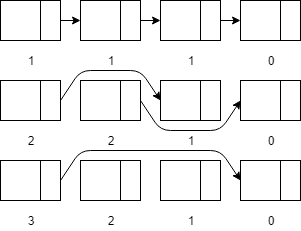
\includegraphics[width=0.5\linewidth]{Chapters/GPU/Algorithms/ListRanking.png} 
    \caption{List ranking}
\end{figure}

\subsection{Euler tour}

R. Tarjan and U. Vishkin introduced the Euler tour technique~\cite{tarjan1985efficient}; the Euler tour is defined as being able from one vertex of the graph to visit every edges exactly twice, in both direction. Hence, it can be easily mapped to a list ranking problem and this technique was used to solve many theoretical problems leading to several and various results to trees.

The bottom idea is that we can use the prefix sum algorithm through the Euler tour technique. This allows us to represent our tree structure as a flat collections of elements and apply our more advanced operations on all the elements without worrying on the accesses.

\subsection{Tree contraction}

Tree contraction was introduced by G .L. Miller and J. H. Reif in 1989~\cite{miller1989parallel} and has been used to design many and efficient parallel algorithms due to the possibility to represent the problems as a tree. The algorithm requires two primary operations:

\begin{itemize}
    \item Rake which removes all the leafs of a tree (merging childless nodes together).
    \item Compress consists to identify every vertex $v_{i}$ with $v_{i+1}$ when $i$ is odd and $v_{i}$ has only one child which is not leaf.
\end{itemize}

Both operations are successively repeated until the tree is reduced to one and unique node. The maximal number of iterations needed is bounded by $O(\log N)$. This helps us to work with any tree and guarantee $O(\log N)$ operations even with degenerated cases like linked list.

Many algorithms are based on this algorithm, the \textit{Arithmetic Expression Evaluation}, the \textit{Tree isomorphism} or to find the \textit{3-connected components} of a graph~\cite{miller1991parallel}. Those present a complexity in $O(\text{sort}_{P}(N))$ with $P \leq \frac{N}{B^{2} \log B}$.

\subsection{Lowest common ancestors}

The lowest common ancestor (LCA) of two nodes $v$ and $w$ in a tree $T$ is the lowest (i.e. deepest) node that has both $v$ and $w$ as descendants.

D. Harel and R. E. Tarjan showed that LCA queries can be answered in constant time after only linear preprocessing of the tree through \textit{Heavy path decomposition}~\cite{harel1984fast} but that data structure may be hard to implement. Arge et al., proposed to consider a simple $(\frac{M}{B})$-ary search tree\index{B-tree} which guarantees $O(\log_{\frac{M}{B}} \frac{N}{B})$ levels. The $K$ queries are treated after sorting the items, so that all of the queries can be answered by scanning the search tree a constant number of times through reduction of the problem to range minimum query (RMQ). The complexity is thus expressed as $O((1 + \frac{K}{N}) \text{sort}_{p}(N))$ I/Os.

\begin{figure}[!htb]
    \centering
    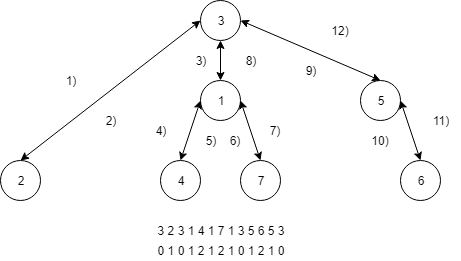
\includegraphics[width=0.8\linewidth]{Chapters/GPU/Algorithms/EulerTour.png} 
    \caption{LCA - RMQ: Euler tour}
\end{figure}

% Sparse table
% node prefix and suffix minima => http://wwwmayr.in.tum.de/lehre/2013WS/pa/split/sec-Tree-Algorithms-handout.pdf
% http://madalgo.au.dk/fileadmin/madalgo/OA_PDF_s/C269.pdf

\subsection{Connected and biconnected components, ear decomposition and minimum spanning tree}

Arge et al.~\cite{arge2010parallel} propose also many theoretical results in links to these problems:

Finding a minimum spanning tree, the connected components, the biconnected components and performing the ear decompositon can all be solved on the undirected connected graphs $G = (V, E)$ can be solved in $O(\text{sort}_{p}(|V|) + \text{sort}_{p}(|E|) \log(\frac{|V|}{PB})$ I/Os in the PEM model using up to $P \leq \frac{|V |+|E|}{B^{2} \log^{2} B}$ processors.

If the graph is sparse and closed under contraction, the connected components, the minimum spanning tree (if G is connected), the biconnected components and ear decomposition (if G is biconnected) can be computed in $O(\text{sort}_{p}(|V|))$ I/Os with $P \leq \frac{|V |+|E|}{B^{2} \log^{2} B}$.

Those results are extension of the work of Chiang et al.~\cite{chiang1995external} in external memory model. They relied on many other algorithms which would be out of the scope. These algorithms are often based on the Minimum Spanning Forest problem, where we divide the graphs among the processors. They all define a priority queue based on the weights of the concerned nodes and apply a Prim-like algorithm~\cite{arge2000external}. N. Zeh proposes a work in which he gathers many results with demonstrations and detailed explanations for the sequential I/O algorithms~\cite{zeh2002efficient}.

\section{Geometric problems}

A classical set of problems and algorithms are the geometric ones. They appear in a wide range of problems, often in somewhat concealed forms, but offer frequently elegant solutions. Many of the sequential algorithms are based on divide-and-conquer and lead in a relatively straightforward manner to efficient parallel algorithms.

\subsection{Interval stabbing counting and 1-D range counting}

Given $I$, a set of intervals, and $S$, a set of points on the real line, with $|I| + |S| = N$. The \textit{interval stabbing counting} problem consists to compute the number of intervals containing each point of S. The \textit{1-D range counting problem}, is the opposite, to compute the number of points contained in each interval.

These two problems can be solved in $O(\text{sort}_{p}(N))$ I/Os. But, in the case where the inputs are already sorted by their value for $S$ and by the end of the interval for $I$, interval stabbing counting is in $O(\frac{N}{PB})$ and the 1-D range counting is bounded by $O(\text{sort}_{p}(|I|) + \frac{|S|}{PB})$.

The idea to count the number of intervals containing a point is to assign a weight of $1$ to every left interval endpoint, a weight of $-1$ to every right one and $0$ to every point in $S$. And then apply a prefix sum in $O(\frac{N}{PB})$.

On the other hand, compute the number of points within the intervals is the difference of the prefix sums of its endpoints after assigning a weight of 1 to every point and 0 to every interval endpoint. The two prefix sums are trivial, but the difference is not. We must first extract the set of interval endpoints from the point list using a compaction operation and sort the resulting list to store the endpoints of each interval consecutively; this operation takes $O(\text{sort}_{p}(|I|) + \frac{|S|}{PB})$. They also came up with an optimal algorithm in $O(\frac{(N + K)}{PB} + \log P)$ when $P \leq min(\frac{N}{B \log^{2}N}, \frac{N}{B^{2}})$ and where $K$ are the queries but which is way more complex~\cite{ajwani2011optimal}.

\subsection{2-D weighted dominance counting}

The problem is posed as follows: Given a set of points ($q \in S$), each of them associated with a weight, the goal is to compute the total weight of all points 2-dominated by each point in S. The 2-D dominance is defined as such: given two points in the plane $q_{1} = (x_{1}, y_{1})$ and $q_{2} = (x_{2}, y_{2})$, $q_{1}$ 1-dominates $q_{2}$ if $y_{1} \geq y_{2}$ and 2-dominates if it both 1-dominates and $x_{1} \geq x_{2}$.

This problem looks quite surprising, but some others reduced to it~\cite{atallah1986sweeping}. The problem, by it-self, can be solved using $O(\text{sort}_{p} (N))$ I/Os in the PEM model.

The first step of the algorithm consists to sort the points along their x-coordinates and partition this collection into vertical slabs $\sigma_{i}$, each containing $\frac{N}{P}$ points. Then, in parallel, we sort the slabs along the y-axis, we get a new list $U(\sigma_{i})$ and we associate to each one two new weights: $W^{1}_{\sigma_{i}}(q)$ and $W^{2}_{\sigma_{i}}(q)$ which are the total weights of the points within $\sigma_{i}$ that $q$ 1- and 2-dominates, respectively.
It then remains to group up the information. The obtained lists can be merged together using a d-way cascading merge procedure where we have a d-ary tree where the leaves are the $\sigma_{i}$. At each tree node $v$, we compute a new y-sorted list $U(v)$ which is the result of the subnodes. While we are doing this operation, we can also compute the new weights $W^{1}_{v}(q)$ and $W^{2}_{v}(q)$ since those can be expressed as the sum of their predecessors in the merged lists. At the end, the root $r$ of the tree has $U(r) = S$ and $W^{2}_{r}(q)$ is the total weight of the dominated points~\cite{ajwani2010geometric}.

\subsection{Distribution sweeping}

In computational geometry, a sweep line or plane sweep is an algorithmic tool which is used to solve many problems. One can imagine that a line is swept accross the plane and stops at some points. The idea is to construct the solution bit by bit while we meet new points to finally produce our solution. This concept has been extended to parallel problems in 1985 and it is more well-knowed as distributed sweeping~\cite{atallah1986sweeping}. It can be rougly expressed as subdividing recursively the plane into slabs such that they contain about the same number of elements, with $min(\sqrt{\frac{N}{P}}, \frac{M}{B})$. But this framework may be hard to implement due to parallelism of line sweeping and due to the expected good load balancing if we consider output sensitive algorithms~\cite{ajwani2013empirical}.

D. Ajwani, N. Sitchinava and N. Zeh propose an optimal algorithm to solve three problems: \textit{Orthogonal line segment intersection}, \textit{Batched orthogonal range reporting} and \textit{Rectangle intersection reporting}~\cite{ajwani2011optimal}. The optimal complexity achieved is in $O(\text{sort}_{p}(N) + \frac{K}{PB})$ but is really complex. It can be easier to duplicate horizontal segments which cross different partitions and then apply the standard algorithm, this would lead to a $O(\text{sort}_{p}(N + K))$ where $K$ is the number of duplicates segments.

To realize such results, they extended the external memory data structure called \textit{Buffer Tree} which provide amortized complexity for queries and which can be used as a priority queue~\cite{arge2003buffer}. This structure can be seen a specialization of the B-trees, the classical balanced trees, as R-trees are for range queries. They assign $\Theta(\frac{1}{PB} \log_{\frac{M}{B}} \frac{N}{B})$ credits to each operations and modify the structure to maintain the invariant when the buffer is full, it is then emptied and the sub-nodes are impacted~\cite{sitchinava2012parallel}.

They also propose a solution to the problems of: \textit{Lower envelope of a set of non-intersecting 2-D line segments}, \textit{Convex hull of a 2-D point set}, and \textit{maxima of a 3-D point set}. All of these are in $O(\text{sort}_{p} (N))$, provided $P \leq \frac{N}{B^{2}}$ and $M = B^{O(1)}$. Convex hull simply consists to subdivide the problem into pair wise convex hull problems through Graham Scan technique and then compose the solution finding the tangent~\cite{atallah1988parallel}. The other problems can be solved using a technique close to 2-D weighted dominance through clever change in the labels~\cite{atallah1986efficient}.


% View http://web.mit.edu/6.976/www/handout/valiant2.pdf

\section{Matrix algorithms}

While considering matrix algorithms, it is worth to consider the way the elements are laid out in memory. Sparse matrices are designed such that only non-zero entries are stored  as a triple of value and row, column. For a dense matrices, we usually distinguish the three following layouts:
\begin{itemize}
    \item Column major layout: The records are ordered by column first, and by row index within a column.
    \item Row major layout: The records are order row-wise first, and column-wise within a row.
    \item Recursive layout or zig-zag: Such layouts are often helpful to construct efficient cache-oblivious algorithm. Many applications involve (recursive) space filling curves to define the ordering of records.
\end{itemize}

\subsection{Matrix compaction and transposition}

The problem consists to transpose a matrix A of total size $N_{x} \times N_{y} = N$, composed as $P$ rows $A_{i}$ divided in $d$ sub-arrays, such that it procudes a new matrix $A^{'}$,
with $d$ rows and $P$ subdivisions. The segmentation is given through a matrix $M$ whose dimensions are 
$P \times d$ where $M[i, j]$ gives the size of the subarray.

A. Aggarwal and J. S. Vitter point out that transposition is a special case of permutation. Indeed, one can imagine that the matrix is broken down into several subgroups that will be used to create the final result. And then, it is necessary to merge the results through a fusion procedure, with the intuition that the same subgroups remain together. Hence a natural bound, for dense matrix, of $\Omega(\frac{N}{PB} \log_{d} \text{min}(B, N_{x}, N_{y}, \frac{N}{B}))$ with $d = \text{max}(2, \text{min}(\frac{M}{B}, \frac{N}{PB}))$~\cite{greiner2012sparse}. Cantazaro et al. propose another solution to this problem which has the advantage to be bank-conflict free~\cite{catanzaro2014decomposition}.

\begin{figure}[!htb]
    \centering
    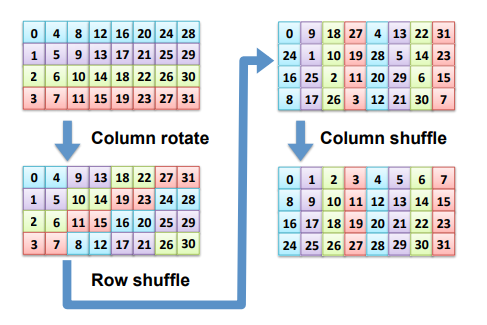
\includegraphics[width=0.8\linewidth]{Chapters/GPU/Algorithms/Transposition.png} 
    \caption{Catanzaro transposition - image extracted from Catanzaro et al.~\cite{nobile2014cutauleaping}, doi:10.1145/2692916.2555253}
\end{figure}

\subsection{Matrix-vector multiplication}

Performing a \textit{Sparse matrix-vector multiplication} can be bound in $\Omega(\frac{wH}{PB})$ with $H$ the number of non-empty entries and $w$ the number of vectors to multiply. And computing the bilinear form adds a factor of $O(\log ~ \text{min}(\frac{\sqrt{N}}{B}, \frac{P}{w}))$ since we can compute the partial scalar product when we are writing the resulting vector of the matrix multiplication and then gather the result~\cite{greiner2012sparse}. This extends the work of Bendal et al.~\cite{bender2010optimal} to parallel machines. Those sparse notions have a lot of application since they can have deep connection with graph problems~\cite{yang2015fast}.

\subsection{Matrix multiplication}

If we apply the standard matrix multiplication algorithm for two dense matrices, with the first matrix in row-major order and the second in column-major, for each element, we would have to do two scans, which would end up in $O(\frac{N^{3}}{PB})$ which is not optimal. Indeed, it is feasible to achieve $\Theta(\frac{N^{3}}{BP\sqrt{M}})$~\cite{ballard2012graph} for the classical algorithm, this coincides with one of the first result achieved by Hong and Kung. One should remark that multiple rows and columns are read several times, leading to inefficiency. The solution consists to store the elements of the matrices recursively, each time subdividing the 4 corners one after the other with a layout like $\text{layout}(Z) = \text{layout}(Z_{11})\text{layout}(Z_{12}) ... \text{layout}(Z_{22})$.

The complexity can be described by this system:
$$
\left\{
    \begin{array}{ll}
        MT(N) = 8MT(\frac{N}{2}) + O(\frac{N^{2}}{B}) \\
        MT(\sqrt{\frac{M}{3}}) = O(\frac{M}{B})
    \end{array}
\right.
$$

Indeed, each corner of the resulting matrix is obtained as the sum of the product of two sub-matrices, we have 4 corners with 2 products. The sums are independent of the recursion and cost $O(\frac{N^{2}}{B})$ since we scan along $X$ and $Y$. Finally, when the submatrices can be entirely contained in the cache\index{Cache}, and as they are stored continuously, the worst case is to go through all these blocks\index{Block}, $O(\frac{M}{B})$. Now, due to master theorem, we need to count the number of leaves, since the sum costs more than the recursion, there are thus $8^{\log N / \sqrt{M / 3}} = (N / \sqrt{M / 3})^{3}$ leaves. The total cost is finally:

$$ (\frac{N}{\sqrt{M / 3}})^{3} O(\frac{M}{B}) = \Theta(\frac{N^{3}}{M^{3/2}}) O(\frac{M}{B}) = \Theta(\frac{N^{3}}{B\sqrt{M}}) $$

%MT(N) = 8MT(N/2) + O(N^2 / B)
%Base case = MT(sqrt(M / 3)) => cost M/B
% There are 8^{log N / sqrt(M / 3)} leaves which is (N / sqrt(M / 3))
% Multilpy this by M / B
% https://youtu.be/CSqbjfCCLrU?t=1h16m53s


Sparse-dense matrix multiplication has a complexity dependent of the number of processors that we may offer, $\Omega(\frac{H\sqrt{N_{z}}}{PB\sqrt{M}})$ with $P \leq
HN_{z} / M^{\frac{3}{2}}$. Sparse-Sparse multiplication is still an open question, but we know that the complexity is bound by $\Omega(\frac{H_{1}H_{2}N}{PB} \log \frac{N}{\text{min}(H_{1}, H_{2}) B)})$ where $H_{1}$ (respectivelly $H_{2}$) is the average number of non-zero elements per column. Ballard et al.~\cite{ballard2011minimizing} regroup the results for the classical matrix decomposition (SVD, LU, ...).


\section{Sort}

Sorting is a building block for many algorithms. Indeed, countless of those take for precondition a sorted collection. Hence, it is important to try to achieve the best performances possible to make benefit all the others. It is also intented to design them such that they benefit the most from the hardware. GPUs are thus good candidates to gain efficiency since we can perform many operations at the same time, like comparisons.

One of the first results achieved for the PEM model of computation was the complexity bound of this problem which are inbetween $\Omega(\text{min}(\frac{N}{P}, \frac{N}{PB} \log_{\frac{M}{B}} \frac{N}{B}) + \log \frac{N}{B})$ and $O(\frac{N}{PB} \log_{\frac{M}{B}} \frac{N}{B})$ with $P \leq \frac{N}{B^{2}}$ and $M = B^{O(1)}$~\cite{arge2008fundamental}.

\subsection{Sorting networks}

One classical notion when talking about parallel sorting is the use of sorting networks, with the classical Batcher's odd-even mergesort or bitonic mergesort~\cite{batcher1968sorting}. But, even though, these sorting networks are not optimal, they provide good runtimes since they can be efficiently hardware-implemented. Hence, they grant low constant factors, good locality and no bank conflicts but they can not be used practically to sort large arrays. A certain type of sorting network is also at the origin of the complexity of permutation in External Memory model~\cite{jia1981complexity}.

\subsection{Shearsort}

Shearsort can be viewed as an analogue to the sorting networks but viewing the problem as a matrix. Elements are first sorted by rows, alternating between ascending and decreasing. Then, follow by sorting column-wise and repeat those two steps up to $\Theta(\log(N))$ times~\cite{sitchinava2013provably}. It also benefits from being bank-conflict free.

\subsection{Radix sort}

% http://www.cs.ucr.edu/~stelo/cpm/cpm15/28_Karkka.pdf

When we are interested in the task of sorting elements, we have to be aware that we intend most of the time comparison-based. But there are some sort algorithms which do not rely on that and use other kind of information. One of the most well known is the radix sort for integer-like elements. It consists to use the propriety of the elements to directly sort them, hence it only keeps to do it in a clever way to avoid scattering and scanning~\cite{satish2009designing}.

\subsection{Distribution sort}

The distribution sort consists to partition the unsorted set of $N$ elements into $d$ buckets, each being recursively sorted and concatenated to obtain the final result, it can be viewed as a generalization of the quicksort. The algorithm, by it-self, randomly sample elements of the data to get $\sqrt{d}$ pivots, partition the data and calls it-self on those subsets. When there are not enough data left to recurse one again, we perform a simple sort. One heuristic is used to determine the pivots, in link to the theoretical results of A. Aggarwal and J.S. Vitter~\cite{aggarwal1988input}, it consists to sample a part of the elements that we want and construct on them our pivot distribution.

Its complexity is in $O(\frac{N}{PB} \log_{\frac{M}{B}} \frac{N}{B})$ when the number of elements $N \geq PB$ and $M \geq B^{c}$ for some $c > 1$. Otherwise, its expression is way more complex~\cite{arge2008fundamental}.

\subsection{Multiway merge sort}

Casanova et al. proposed in 2017, a new algorithm called: \textit{Multiway Mergesort} (MMS)~\cite{casanova2017efficient}. It is the first sorting algorithm for the GPU that is asymptotically optimal in terms of global memory accesses and without any bank conflicts in shared memory. This algorithm intervenes while trying to solve two problems. Indeed, previous algorithms benefited from coalesced memory accesses but they were not trying to reduce the total number of accesses and were less cautious with the banks which may appear in the merging phase.

The proposed algorithm is based on the classical notion of merge sort, which can be parallelised efficiently using partitioning~\cite{satish2009designing}. Instead of two sublists merged together multiple ones are treated at the same time. To allow parallelism, it also uses a notion of partitioning which splits some sorted list by the median pivot. Then, it tries to merge efficiently avoiding bank conflicts and trying to maximize memory coalescing. It remains to sort basis elements which will be source of the recursion for the multiway merging algorithm, this is achieved by a shearsort~\cite{sitchinava2013provably}.

Let us return a little on the complexity of the classic merge sort, with the fusion of two lists at once. The complexity is described by this system:
$$
\left\{
    \begin{array}{ll}
        MT(N) = 2MT(\frac{N}{2}) + O(\frac{N}{B}) \\
        MT(M) = O(\frac{M}{B})
    \end{array}
\right.
$$

Since we recurse on both sides and, to merge two lists, we need to perform one scan on two arrays, so $O(\frac{N}{B})$. Now, we remark that the height of the recursion is bounded by $O(\log N - \log M) = O(\log \frac{N}{M})$ since once we reach the cache\index{Cache} size, everything becomes essentially free. Finally, the amount of work is the same for each level of the tree, hence $O(\frac{N}{B} \log \frac{N}{M})$. But this is not optimal, since we don't use efficiently all the cache\index{Cache} available to us when merging the lists, we could merge up to $\frac{M}{B}$ lists at the same time. The coefficient ``$2$'' becomes $\frac{M}{B}$ and we finally reach the optimal bound of $O(\frac{N}{B} \log_{\frac{M}{B}} \frac{N}{B})$. Now, to adapt the result to parallelism, we just need to find out a way to split the data and merge the lists in $O(\frac{N}{PB})$. But merging lists is not as trivial as it sounds~\cite{green2012gpu}.